% Figure 4: Disagreement-Based Selective Triage
% Standalone TikZ -- compiles independently to PDF
\documentclass[tikz,border=10pt]{standalone}
\usepackage{tikz}
\usetikzlibrary{shapes.geometric, arrows.meta, positioning, calc, fit, backgrounds}
\usepackage{amsmath}

% ── Colour palette (consistent across all figures) ──────────────────────────
\definecolor{processblue}{HTML}{4A90D9}
\definecolor{processbluedark}{HTML}{2C6FAC}
\definecolor{alertred}{HTML}{E74C3C}
\definecolor{alertreddark}{HTML}{C0392B}
\definecolor{cleargreen}{HTML}{27AE60}
\definecolor{cleargreendark}{HTML}{1E8449}
\definecolor{deferamber}{HTML}{E67E22}
\definecolor{deferamberdk}{HTML}{CA6F1E}
\definecolor{bglight}{HTML}{F0F4F8}
\definecolor{patientteal}{HTML}{1ABC9C}
\definecolor{patienttealdark}{HTML}{16A085}
\definecolor{textdark}{HTML}{2C3E50}
\definecolor{modelpurple}{HTML}{8E44AD}
\definecolor{modelpurpledark}{HTML}{6C3483}
\definecolor{modelnavy}{HTML}{2C3E80}
\definecolor{modelnavydark}{HTML}{1A2550}
\definecolor{computegray}{HTML}{566573}
\definecolor{computegraydark}{HTML}{2C3E50}

\begin{document}
\sffamily
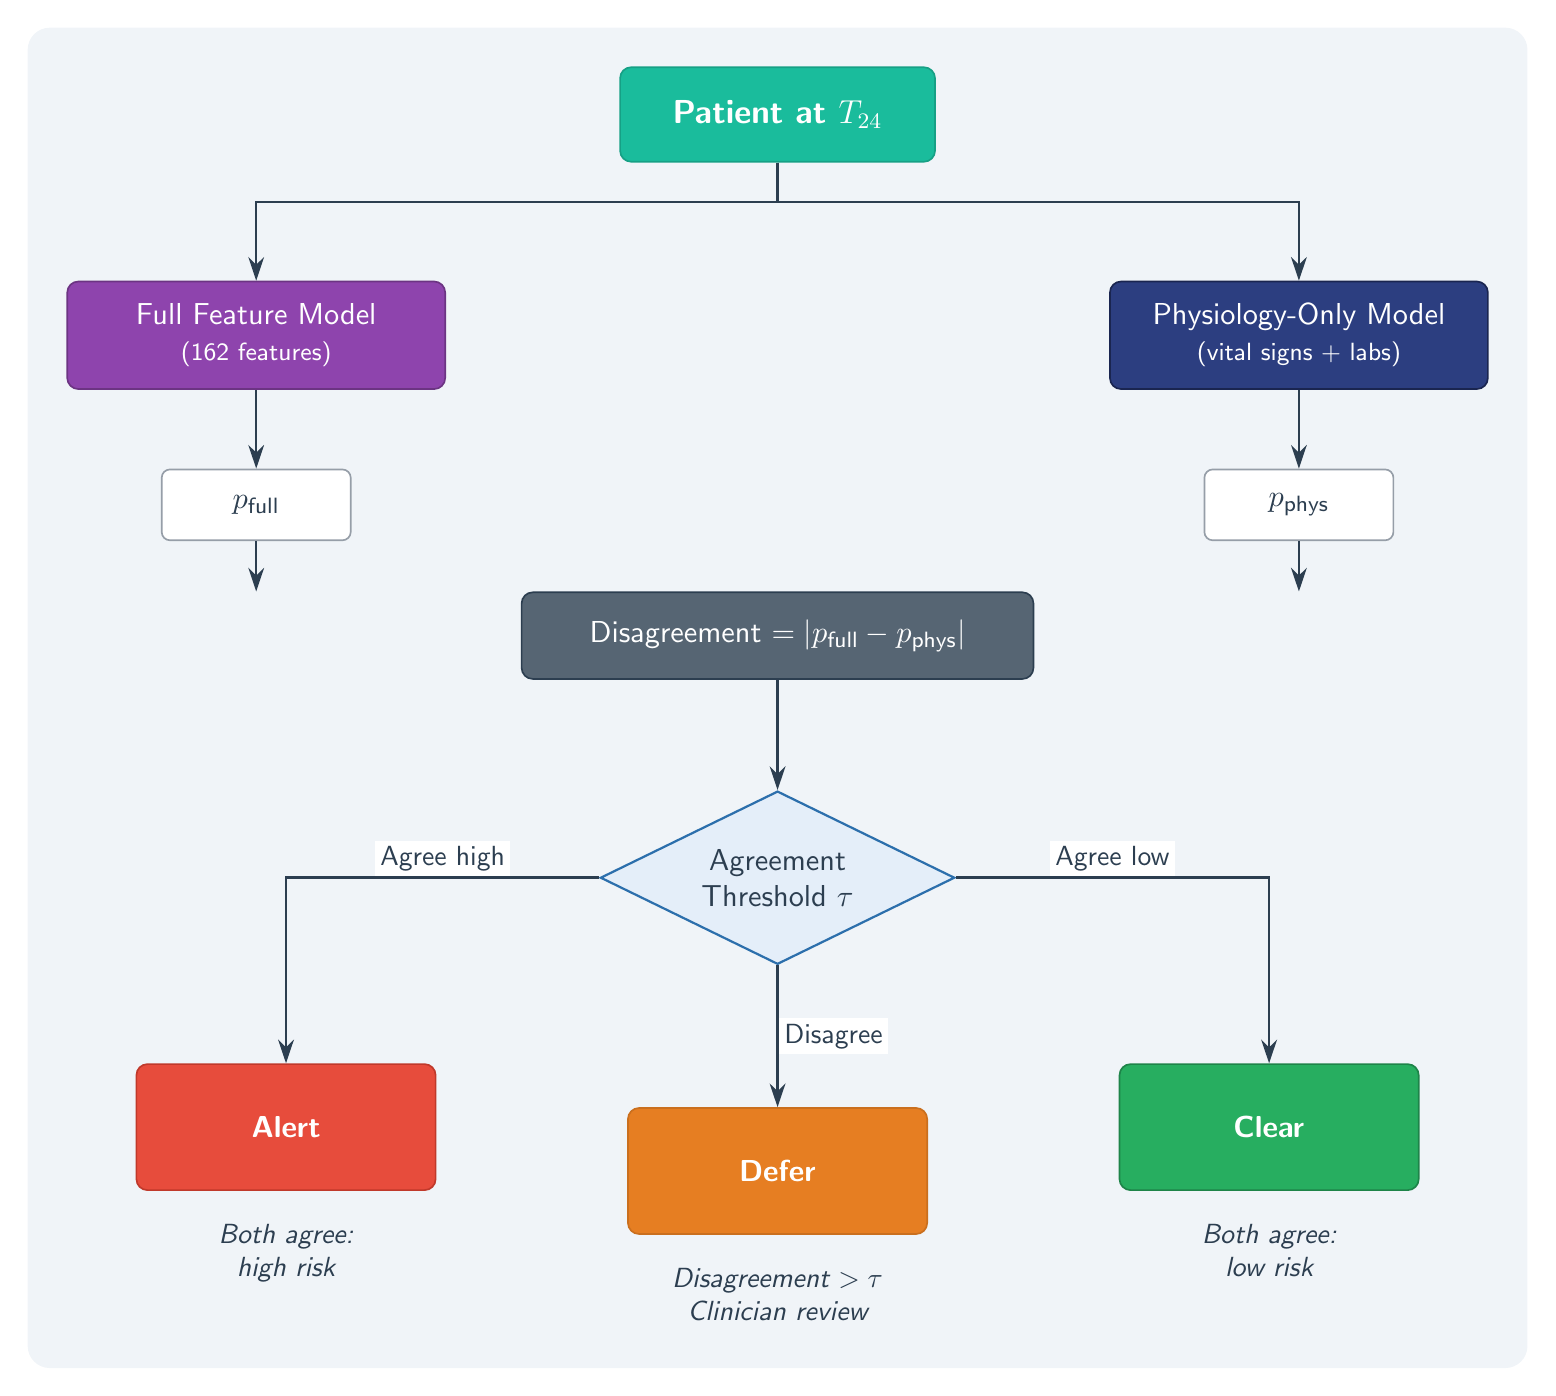
\begin{tikzpicture}[
    % ── Node styles ──────────────────────────────────────────────────────
    base/.style={
        draw, rounded corners=4pt, minimum height=1.1cm,
        font=\fontsize{11}{13}\selectfont\sffamily,
        text=white, align=center, inner sep=8pt,
        line width=0.6pt
    },
    patientnode/.style={
        base, fill=patientteal, draw=patienttealdark,
        minimum width=4cm, minimum height=1.2cm,
        font=\fontsize{12}{14}\selectfont\sffamily\bfseries
    },
    modelA/.style={
        base, fill=modelpurple, draw=modelpurpledark,
        minimum width=4.8cm
    },
    modelB/.style={
        base, fill=modelnavy, draw=modelnavydark,
        minimum width=4.8cm
    },
    probnode/.style={
        draw, rounded corners=3pt, minimum height=0.9cm,
        minimum width=2.4cm,
        font=\fontsize{11}{13}\selectfont\sffamily,
        text=textdark, align=center, inner sep=6pt,
        fill=white, line width=0.6pt, draw=textdark!50
    },
    computenode/.style={
        base, fill=computegray, draw=computegraydark,
        minimum width=6.5cm
    },
    decision/.style={
        draw, diamond, aspect=2.2, minimum width=4.5cm,
        minimum height=2.2cm, inner sep=4pt,
        fill=processblue!15, draw=processbluedark,
        line width=0.8pt,
        font=\fontsize{11}{13}\selectfont\sffamily,
        text=textdark, align=center
    },
    alertbox/.style={
        base, fill=alertred, draw=alertreddark,
        minimum width=3.8cm, minimum height=1.6cm
    },
    clearbox/.style={
        base, fill=cleargreen, draw=cleargreendark,
        minimum width=3.8cm, minimum height=1.6cm
    },
    deferbox/.style={
        base, fill=deferamber, draw=deferamberdk,
        minimum width=3.8cm, minimum height=1.6cm
    },
    actionlabel/.style={
        font=\fontsize{10}{12}\selectfont\sffamily\itshape,
        text=textdark, align=center
    },
    % ── Arrow style ──────────────────────────────────────────────────────
    arr/.style={
        -{Stealth[length=3mm, width=2mm]},
        line width=0.9pt, color=textdark
    },
    arrlabel/.style={
        font=\fontsize{10}{12}\selectfont\sffamily,
        text=textdark, midway, fill=white, inner sep=2pt
    }
]

% ═══════════════════════════════════════════════════════════════════════════
% 1. Patient at top
% ═══════════════════════════════════════════════════════════════════════════
\node[patientnode] (patient) {Patient at $T_{24}$};

% ═══════════════════════════════════════════════════════════════════════════
% 2. Two parallel model branches
% ═══════════════════════════════════════════════════════════════════════════
\node[modelA, below left=1.5cm and 2.2cm of patient] (fullmodel)
    {Full Feature Model\\{\fontsize{9}{11}\selectfont (162 features)}};

\node[modelB, below right=1.5cm and 2.2cm of patient] (physmodel)
    {Physiology-Only Model\\{\fontsize{9}{11}\selectfont (vital signs + labs)}};

% Probability outputs
\node[probnode, below=1.0cm of fullmodel] (pfull) {$p_{\text{full}}$};
\node[probnode, below=1.0cm of physmodel] (pphys) {$p_{\text{phys}}$};

% Arrows: patient → models → probabilities
\draw[arr] (patient.south) -- ++(0,-0.5cm) -| (fullmodel.north);
\draw[arr] (patient.south) -- ++(0,-0.5cm) -| (physmodel.north);
\draw[arr] (fullmodel.south) -- (pfull.north);
\draw[arr] (physmodel.south) -- (pphys.north);

% ═══════════════════════════════════════════════════════════════════════════
% 3. Disagreement computation
% ═══════════════════════════════════════════════════════════════════════════

% Centre point between the two probability nodes
\coordinate (midprob) at ($(pfull.south)!0.5!(pphys.south) + (0,-1.2cm)$);

\node[computenode] (disagree) at (midprob)
    {Disagreement $= |p_{\text{full}} - p_{\text{phys}}|$};

% Arrows: probabilities → disagreement
\draw[arr] (pfull.south)  -- ++(0,-0.4cm) -| (disagree.north -| pfull);
\draw[arr] (pphys.south)  -- ++(0,-0.4cm) -| (disagree.north -| pphys);

% ═══════════════════════════════════════════════════════════════════════════
% 4. Agreement threshold diamond
% ═══════════════════════════════════════════════════════════════════════════
\node[decision, below=1.4cm of disagree] (threshold)
    {Agreement\\Threshold $\tau$};

\draw[arr] (disagree.south) -- (threshold.north);

% ═══════════════════════════════════════════════════════════════════════════
% 5. Three outcome branches
% ═══════════════════════════════════════════════════════════════════════════

% Left — Alert
\node[alertbox, below left=1.8cm and 3.2cm of threshold] (alert)
    {\textbf{Alert}};
\node[actionlabel, below=0.3cm of alert]
    {Both agree:\\high risk};

% Centre — Defer
\node[deferbox, below=1.8cm of threshold] (defer)
    {\textbf{Defer}};
\node[actionlabel, below=0.3cm of defer]
    {Disagreement $> \tau$\\Clinician review};

% Right — Clear
\node[clearbox, below right=1.8cm and 3.2cm of threshold] (clear)
    {\textbf{Clear}};
\node[actionlabel, below=0.3cm of clear]
    {Both agree:\\low risk};

% Diamond to outcomes
\draw[arr] (threshold.west)  -| (alert.north)
    node[arrlabel, pos=0.25, above] {Agree high};
\draw[arr] (threshold.south) -- (defer.north)
    node[arrlabel, right] {Disagree};
\draw[arr] (threshold.east)  -| (clear.north)
    node[arrlabel, pos=0.25, above] {Agree low};

% ═══════════════════════════════════════════════════════════════════════════
% Background
% ═══════════════════════════════════════════════════════════════════════════
\coordinate (bottompad) at ([yshift=-1.2cm]defer.south);
\begin{scope}[on background layer]
    \node[fill=bglight, rounded corners=8pt, inner sep=14pt,
          fit=(patient)(fullmodel)(physmodel)(pfull)(pphys)
              (disagree)(threshold)(alert)(clear)(defer)(bottompad)] {};
\end{scope}

\end{tikzpicture}
\end{document}
